\section{Pohyb a odraz zvuku}

\subsection{Definice zvuku}
\textit{,, Zvuk je mechanické vlnění v látkovém prostředí, které je schopno vyvolat sluchový vjem. Frekvence tohoto vlnění, které je člověk schopen vnímat, jsou značně individuální a leží v intervalu přibližně 16 Hz až 20 000 Hz. Mechanické vlnění mimo tento frekvenční rozsah sluchový vjem nevyvolává, přesto se někdy také označuje jako zvuk. "}\cite{ZvukWikipedie}
\\
\subsection{Pohyb zvuku}
Pokud  se zvuk šíří z bodového zdroje (jak simuluje aplikace) šíří ve formě expandujícího torusu, jehož tloušťka odpovídá vlnové délce. Zvukový impuls vytváří prstencovou strukturu, v níž se střídají oblasti s kladnou a zápornou výchylkou, tak jak ukazuje obrázek č. 1. Body stejně vzdálené od středu tvoří kružnici se stejnou výchylkou, označovanou jako vlnoplocha. Vlnění postupně slábne v důsledku zákona zachování energie, přičemž jeho intenzita klesá nepřímo úměrně druhé mocnině vzdálenosti od zdroje impulsu.\cite{papirNaZvuk}
\newpage
\begin{center}
    \begin{figure}
    \centering
    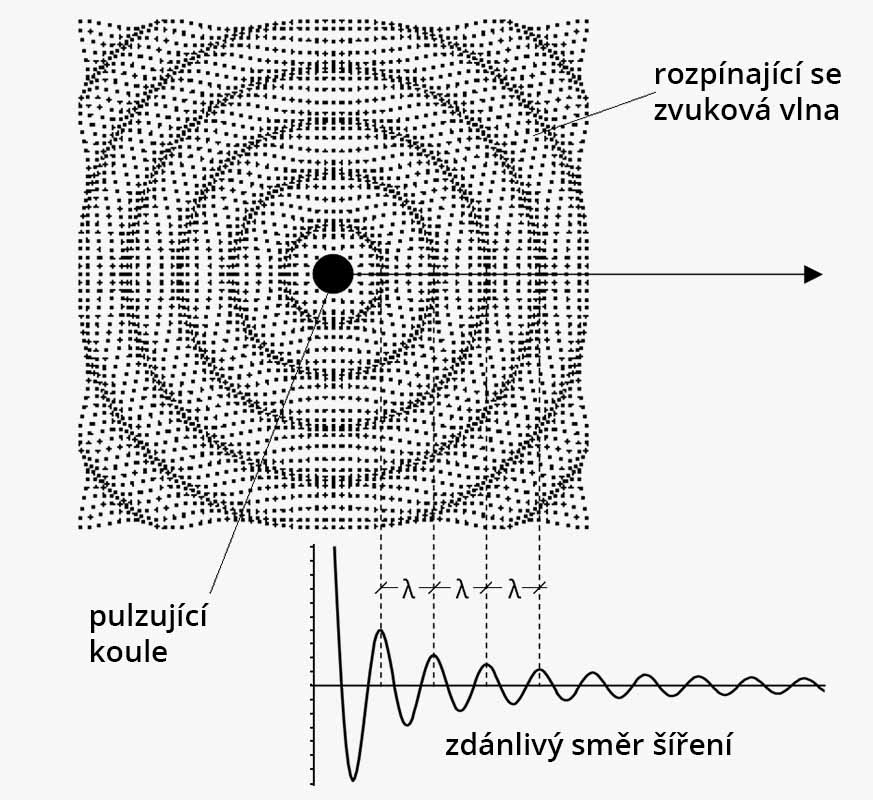
\includegraphics[width=0.5\linewidth]{Obrazky/mic-uni-proximity-fig-2-sound-wave-CZ.jpg}
    \caption{Zvuk šířící se z bodového zdroje\newline
    Zdroj: https://www.audiopro.cz/reseni/co-je-a-jak-se-projevuje-proximity-efekt/}
    \label{fig:enter-label}
\end{figure}
\end{center}



\subsection{Odraz zvuku}
Když zvuk dopadá na stěnu, tak část jeho energie je absorbována zdí a část je emitovaná z jednotlivých bodů zpět do prostoru. Z těchto bodů se zvuk šíří podle zákonu odrazu, který říká, že úhel dopadu je roven úhlu odrazu. To znamená že pokud se zvuk šíří z bodového zdroje, tak odraz zvuku vypadá jako stejná vlna s menší amplitudou, která je osově symetrická vzhledem k dané stěně viz. obrázek č. 2 a 3. \cite{papirNaZvuk}
\begin{figure}
    \centering
    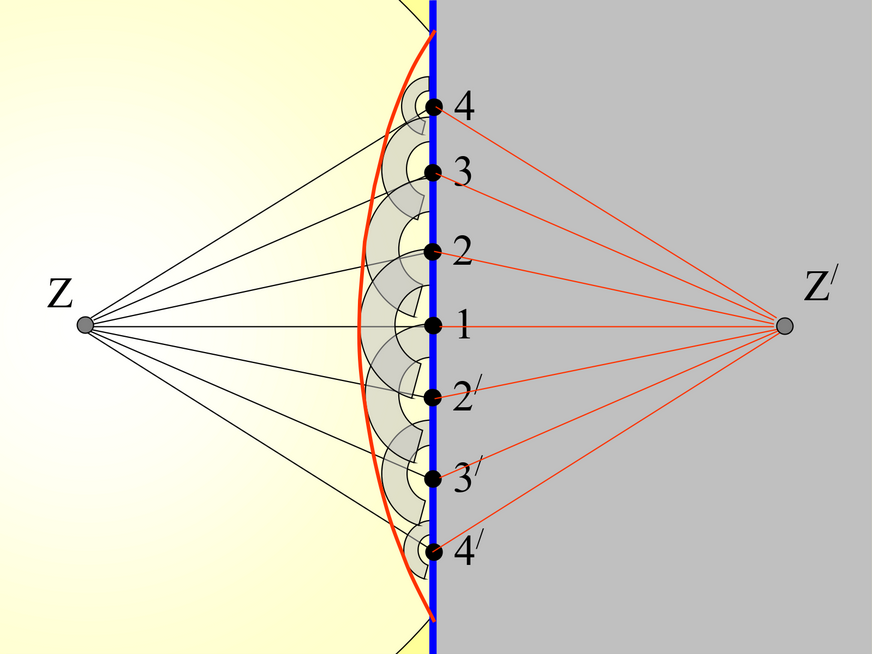
\includegraphics[width=0.5\linewidth]{Obrazky/odraz zvuku s bodama.png}
    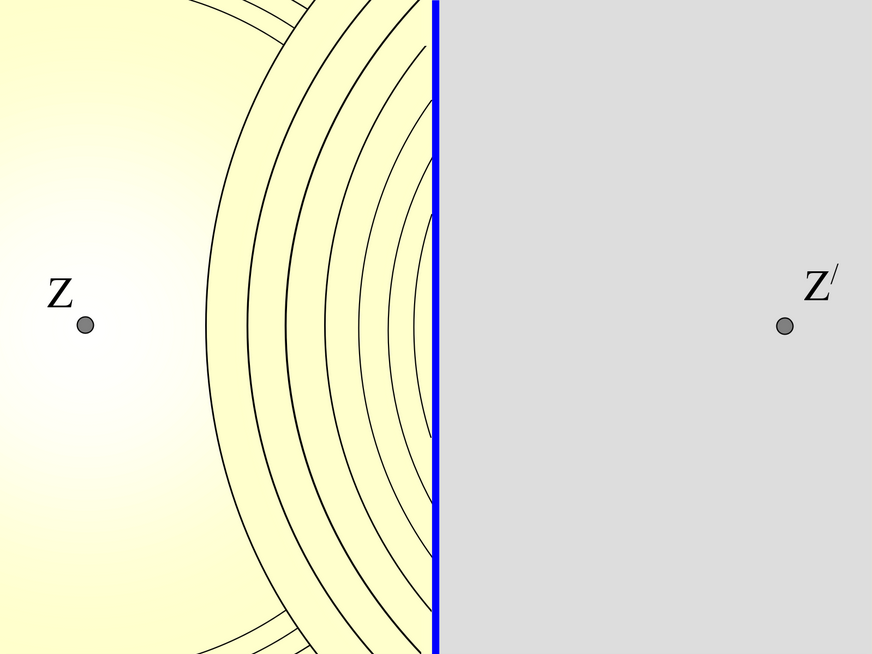
\includegraphics[width=0.5\linewidth]{Obrazky/odraz zvuku bez bodu.png}
    \caption{schema odrazu zvuku s jednotlivými body\\
    Zdroj: Prezentace: Odraz a lom vlnění (PaedDr. Jozef Beňuška  jbenuska@nextra.sk)}
    \label{fig:enter-label}
\end{figure}